% !TeX program = xelatex
\documentclass[a4paper,11pt]{article}
\usepackage[margin=21mm]{geometry}
\usepackage{amsmath,amssymb,booktabs,graphicx,float,longtable,tikz,xcolor}
\usetikzlibrary{arrows.meta,positioning,calc}
\usepackage[colorlinks=true,linkcolor=blue!55!black,urlcolor=blue!55!black]{hyperref}
\setlength{\parskip}{0.4em}\setlength{\emergencystretch}{2em}
\setcounter{tocdepth}{1}
\newcommand{\file}[1]{\texttt{\detokenize{#1}}}
\newcommand{\Kfinal}{\frac{-21.5(s+0.136)(s+0.16)}{s(s+0.0015)(s+0.31)(s+10.7)(s+14.5)}}
\newcommand{\Gplant}{\frac{-88.196939s(s+4.704978)(s+0.06347365)}{D_a(s)}}

\title{AERO5560 Group 8\\Pitch-Rate Inner-Loop Design}
\author{Group 8}\date{20 October 2026}
\begin{document}\maketitle
\begin{abstract}
Three pitch-rate compensators are compared at 200 knots and 300 ft. The selected design achieves a closed-loop bandwidth of 4.237 rad/s, open-loop crossover of 2.017 rad/s, settling time of 1.607 s, steady-state error of 0.116\% and overshoot of 8.897\%. Validation covers adjacent airspeeds, assumed actuator dynamics, parameter uncertainty, nonlinear manoeuvres, measurement noise and digital implementation.
\end{abstract}
\tableofcontents\clearpage
\section{Requirements and Model}
Longitudinal Task 1 requires $G_{q\delta_e}$, a labelled feedback diagram and at least three compensators supported by root-locus, Bode and step-response plots. For a $4^\circ$/s step, the targets are settling within 3 s, steady-state error below 1\%, overshoot below 20\%, elevator within $\pm25^\circ$, frequency in the 2--10 rad/s range, and a stated noise bandwidth of 20 rad/s.

We report open-loop crossover $|L(j\omega_{gc})|=1$ and closed-loop bandwidth $|T(j\omega_{BW})|=10^{-3/20}|T(0)|$ separately [1,2]. Settling uses both final-value and command-centred $\pm2\%$ bands; overshoot is relative to the final value. Tracking metrics use 120 s of linear response, and elevator extrema use 0--10 s. Nonlinear tests use a 5 s step and a 2 s pulse within a 10 s simulation.

Lecture 8-2 (slide 8) and Lecture 9-1 (slides 9 and 17) specify 40 dB attenuation at the noise threshold. At 20 rad/s, the open-loop magnitude is $-41.390$ dB and the closed-loop noise magnitude is $-41.409$ dB. Both satisfy the target. A 20--$10^5$ rad/s sweep confirms at least 40 dB attenuation throughout the checked noise band.

\subsection{Aircraft and Longitudinal Dynamics}
The aircraft has $m=750$ kg, $S=11.9$ m$^2$, $c=0.85$ m and $I_{yy}=1766.52$ kg m$^2$. At $V=102.888$ m/s and $h=91.44$ m, density is 1.21427 kg/m$^3$ and dynamic pressure is 6427.1 Pa. Trim throttle is 0.770317 and elevator is $+0.766074^\circ$.

The fixed-altitude model uses $[\Delta u,\Delta w,\Delta q,\Delta\theta]^T$, fixed throttle and zero gust. Its converged central-difference Jacobians give
\begin{align}
G_{q\delta_e}(s)&=\Gplant,\\
D_a(s)&=(s+4.231362-j3.300400)(s+4.231362+j3.300400)\notag\\
&\quad\times(s+0.0303971-j0.0772921)(s+0.0303971+j0.0772921).
\end{align}
Both longitudinal modes are retained. The short-period mode has $\omega_{n,sp}=5.36629$ rad/s and $\zeta_{sp}=0.788508$.

\section{Bandwidth Selection}
Bandwidth is selected using modal frequency, control authority, noise and actuator response. The selected 4.237 rad/s is below the short-period frequency; its reduced frequency is $c\omega/(2V)=0.01750$, with useful separation from the 20 rad/s noise threshold.

The previous 6.707 rad/s design missed the noise target. Adding a high-frequency pole and retuning the low-frequency poles and zeros reduces bandwidth while preserving tracking. The following fixed-shape gain sweep shows the cost of raising crossover: weaker attenuation and eventually unstable tracking.

\begin{table}[H]\centering\small\caption{Gain-only frequency trade; frequencies in rad/s.}
\begin{tabular}{lrrrrr}\toprule
$\omega_{gc}$ & $\omega_{BW}$ & $t_s$ (s) & OS (\%) & PM (deg) & $|T(j20)|$ (dB)\\\midrule
2.00 & 4.20 & 1.61 & 8.54 & 60.59 & -41.48\\
3.00 & 5.63 & 2.82 & 28.78 & 43.35 & -37.87\\
4.00 & 6.61 & 5.12 & 49.57 & 25.35 & -34.88\\
$\infty$ & $\infty$ & $\infty$ & $\infty$ & $\infty$ & $\infty$\\
$\infty$ & $\infty$ & $\infty$ & $\infty$ & $\infty$ & $\infty$\\
$\infty$ & $\infty$ & $\infty$ & $\infty$ & $\infty$ & $\infty$\\
\bottomrule\end{tabular}\end{table}

\begin{figure}[H]\centering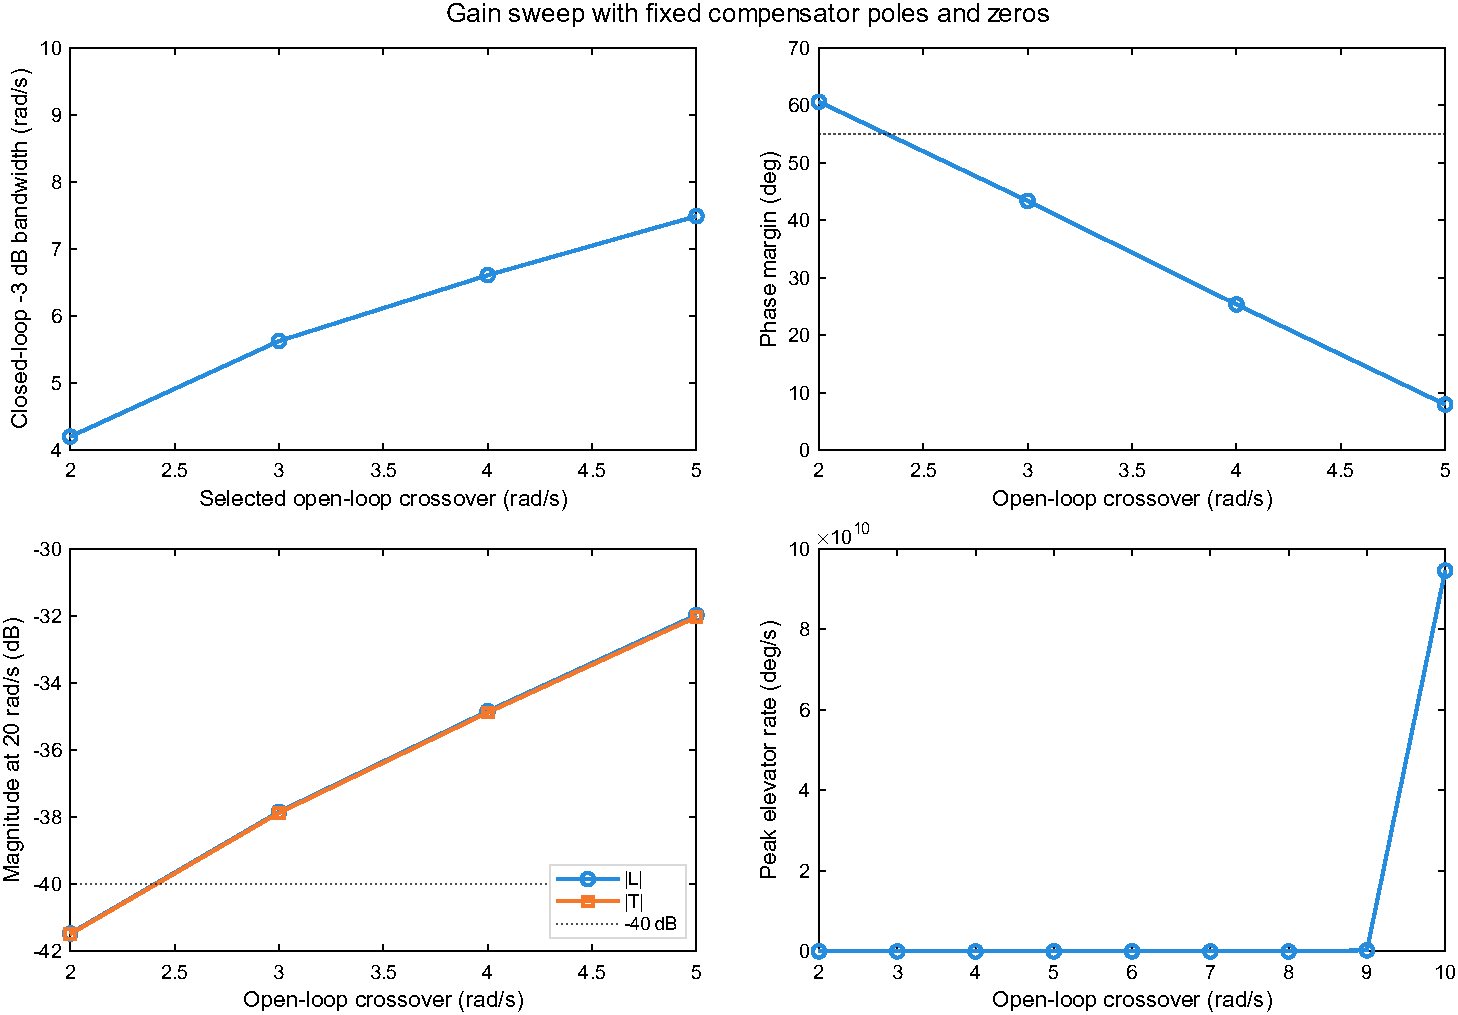
\includegraphics[width=1.0\linewidth]{frequency_trade.pdf}\caption{Gain-only frequency trade.}\end{figure}

A 0.5--1 rad/s starting target for the future vertical-speed loop provides useful separation. The complete nested loop will require a coupled stability check.

\section{Feedback and Sensitivity Functions}

\begin{figure}[H]\centering
\resizebox{\linewidth}{!}{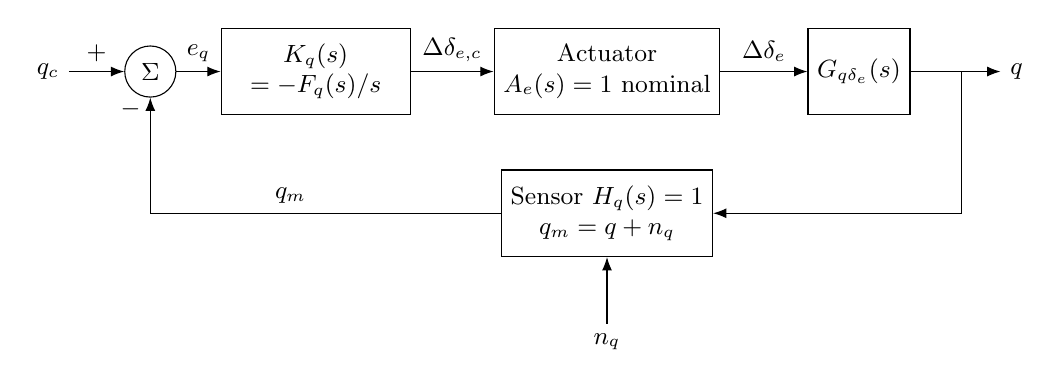
\begin{tikzpicture}[>=Latex,block/.style={draw,minimum height=1.1cm,align=center},font=\small]
\node (r) at (0,0) {$q_c$};
\node[draw,circle,minimum size=6mm] (sum) at (1.3,0) {$\Sigma$};
\node[block,minimum width=2.4cm] (k) at (3.4,0) {$K_q(s)$\\$=-F_q(s)/s$};
\node[block] (a) at (7.1,0) {Actuator\\$A_e(s)=1$ nominal};
\node[block] (g) at (10.3,0) {$G_{q\delta_e}(s)$};
\node (y) at (12.3,0) {$q$};
\draw[->](r)--node[above]{$+$}(sum);
\draw[->](sum)--node[above]{$e_q$}(k);
\draw[->](k)--node[above]{$\Delta\delta_{e,c}$}(a);
\draw[->](a)--node[above]{$\Delta\delta_e$}(g);
\draw[->](g)--(y);
\node[block] (h) at (7.1,-1.8) {Sensor $H_q(s)=1$\\$q_m=q+n_q$};
\draw[->](11.6,0)|-(h);
\draw[->](h)-|node[pos=.3,above]{$q_m$}(sum) node[pos=.95,left]{$-$};
\draw[->](7.1,-3.2)node[below]{$n_q$}--(h.south);
\end{tikzpicture}}
\caption{Pitch-rate feedback. Physical elevator is $\delta_{e0}+\Delta\delta_e$; nominal trim is $+0.766074^\circ$. All dynamic signals use rad and s.}
\end{figure}

Negative plant gain requires negative controller gain. For SISOtool, define
\begin{equation}
P_q=\operatorname{minreal}(-G/s),\qquad K_q=-F_q/s,\qquad L=P_qF_q=GK_q.
\end{equation}
The single external integrator cancels the plant's origin zero in the minimal q channel (Lecture 10-1). SISOtool uses plant $P_q$ and compensator $F_q$. Controller poles and zeros are real; the final loop is strictly proper.
\begin{align}
S&=\frac{1}{1+L},& T&=\frac{L}{1+L}=1-S,& U&=K_qS,\\
q&=Tq_c+GSd_e+Sd_q-Tn_q,&\frac{\Delta\delta_e}{q_c}&=U,&\frac{\Delta\delta_e}{n_q}&=-U.
\end{align}
Here $d_e$, $d_q$ and $n_q$ denote plant-input disturbance, output disturbance and measurement noise. $T$ is the course complementary sensitivity $C$. Numerical ZPK forms are in \file{zpk.txt}.

Since $G\sim-132.596s$ at low frequency, the compensated minimal loop is type 0:
\begin{equation}
\frac{e_{ss}}{q_c}=\frac{1}{1+L(0)},\qquad L(0)>99\ \text{for error below }1\%.
\end{equation}
The final DC loop gain is 859.85 (58.69 dB). Lag compensation raises low-frequency gain while limiting crossover gain.

\section{Compensator Iterations}
\subsection{Iteration 1: Integral Gain}
\begin{equation}K_{q,1}(s)=-0.1961/s.\end{equation}
Crossover is approximately 3 rad/s, but steady-state error is 3.70\% and the slow tail gives 10.92 s settling. Both targets require improvement.
\begin{figure}[H]\centering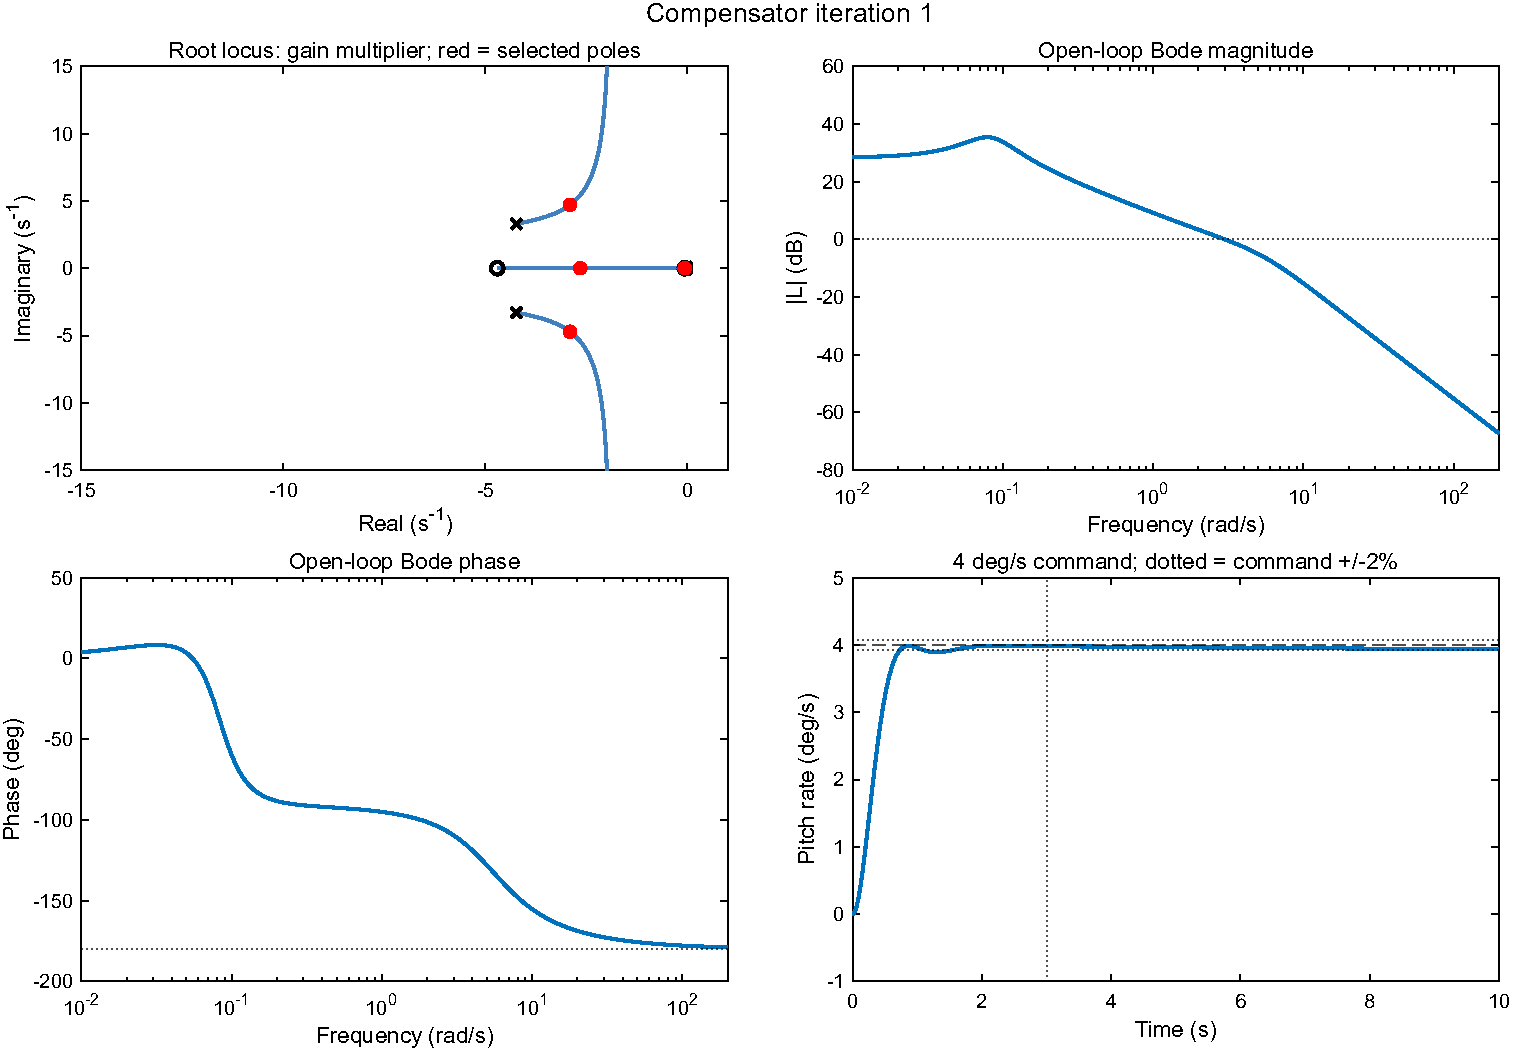
\includegraphics[width=1.0\linewidth]{iteration_1.pdf}\caption{Iteration 1: root-locus detail, Bode and 4 deg/s step; red points mark selected tracking poles.}\end{figure}

\clearpage\subsection{Iteration 2: Lag and Roll-Off}
\begin{equation}K_{q,2}(s)=\frac{-5.835(s+0.5)}{s(s+0.1)(s+30)}.\end{equation}
The lag zero/pole ratio of five reduces steady-state error to 0.77\%. Overshoot remains below 20\%, but phase loss and slow dynamics leave settling at 4.55 s.
\begin{figure}[H]\centering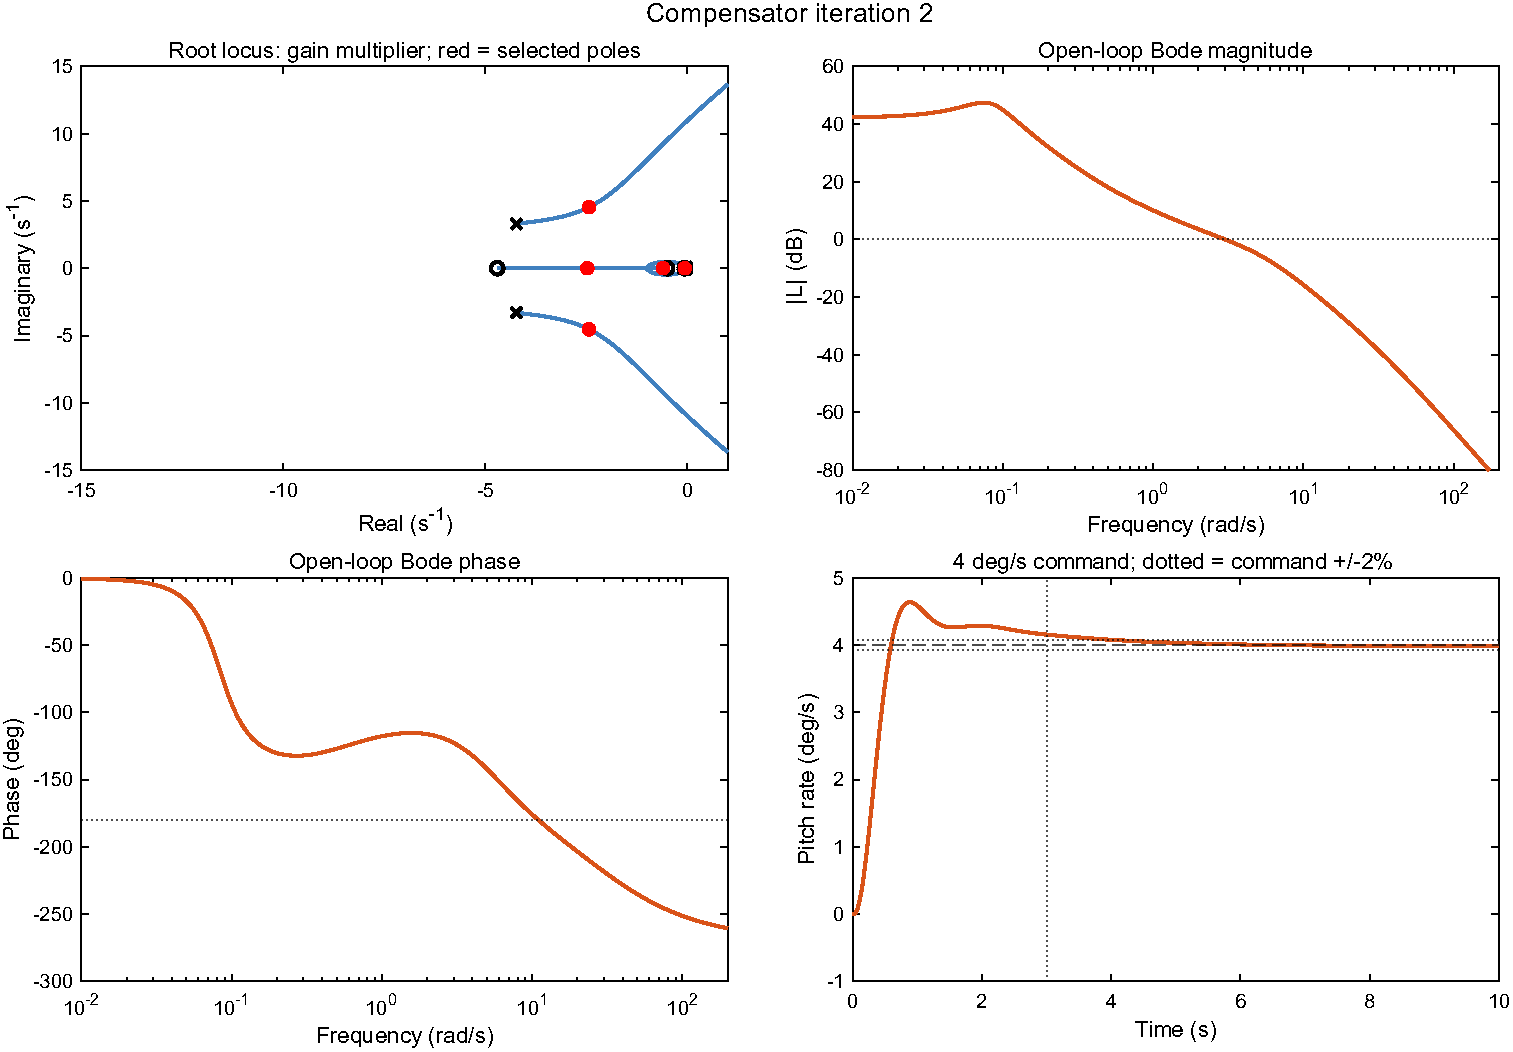
\includegraphics[width=1.0\linewidth]{iteration_2.pdf}\caption{Iteration 2: root-locus detail, Bode and 4 deg/s step; red points mark selected tracking poles.}\end{figure}

\clearpage\subsection{Iteration 3: Low-Frequency Compensation and Noise Roll-Off}
\begin{equation}\boxed{K_q(s)=\Kfinal.}\end{equation}
The SISOtool compensator is
\begin{equation}F_q(s)=\frac{21.5(s+0.136)(s+0.16)}{(s+0.0015)(s+0.31)(s+10.7)(s+14.5)}.\end{equation}
Low-frequency compensation supplies DC gain; poles at 10.7 and 14.5 rad/s supply the additional noise roll-off. After origin cancellation, the open loop has eight poles and four zeros. Parameters were refined against the nominal model, retrimmed 180-knot model and assumed 50 ms actuator, then simplified, rounded and rechecked.
\begin{figure}[H]\centering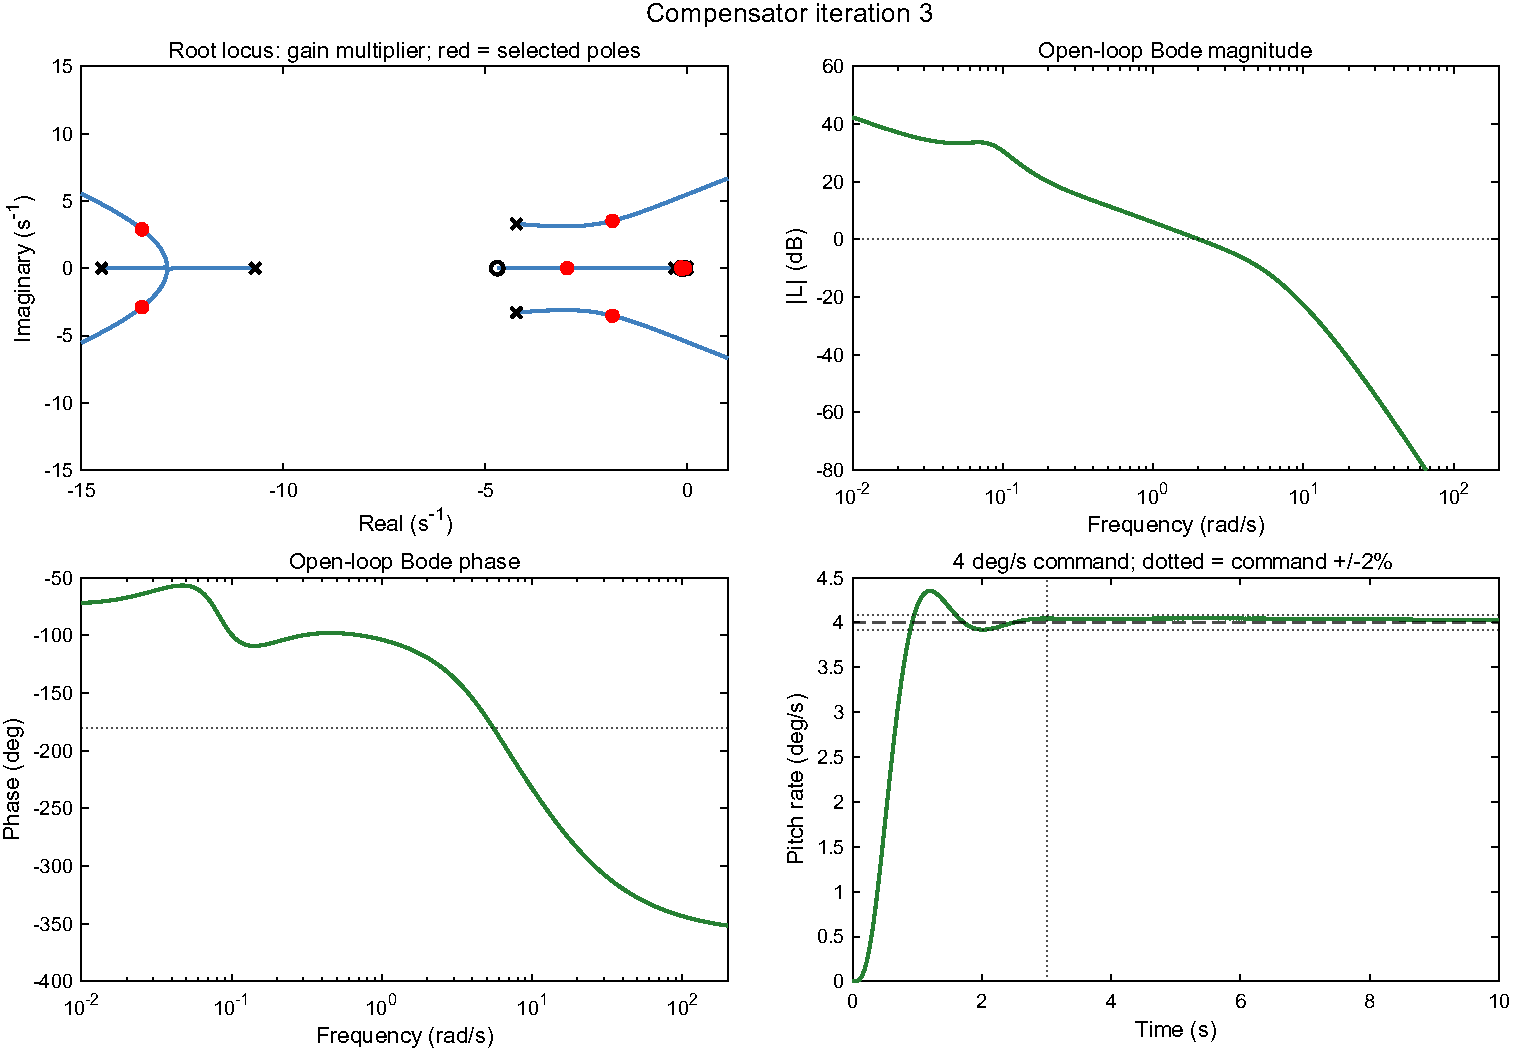
\includegraphics[width=1.0\linewidth]{iteration_3.pdf}\caption{Iteration 3: root-locus detail, Bode and 4 deg/s step; red points mark selected tracking poles.}\end{figure}

\clearpage\subsection{Performance Comparison}
\begin{table}[H]\centering\small\caption{Three compensator iterations; a dash denotes no explicit assignment threshold.}
\begin{tabular}{lrrrr}\toprule
Metric & 1 & 2 & 3 & Target\\\midrule
$\omega_{BW}$ (rad/s) & 5.211 & 5.645 & 4.237 & 2--10\\
$\omega_{gc}$ (rad/s) & 3.000 & 3.000 & 2.017 & 2--10\\
$t_s$, final (s) & 10.919 & 4.546 & 1.607 & $\leq3$\\
$t_s$, command (s) & $\infty$ & 3.938 & 1.602 & $\leq3$\\
SSE (\%) & 3.703 & 0.770 & 0.116 & $<1$\\
Overshoot (\%) & 3.516 & 16.787 & 8.897 & $<20$\\
PM (deg) & 70.418 & 57.155 & 60.301 & --\\
GM (dB) & $\infty$ & 17.419 & 10.806 & --\\
$|T(j20)|$ (dB) & -26.841 & -28.595 & -41.409 & $\leq-40$\\
$|L(j20)|$ (dB) & -27.220 & -28.885 & -41.390 & $\leq-40$\\
\bottomrule\end{tabular}\end{table}

Steady q is 3.9954 deg/s for a 4 deg/s command. Over 0--10 s, absolute elevator is 0.4194--0.7661 deg and peak rate is 0.478 deg/s, leaving substantial position margin.
\begin{figure}[H]\centering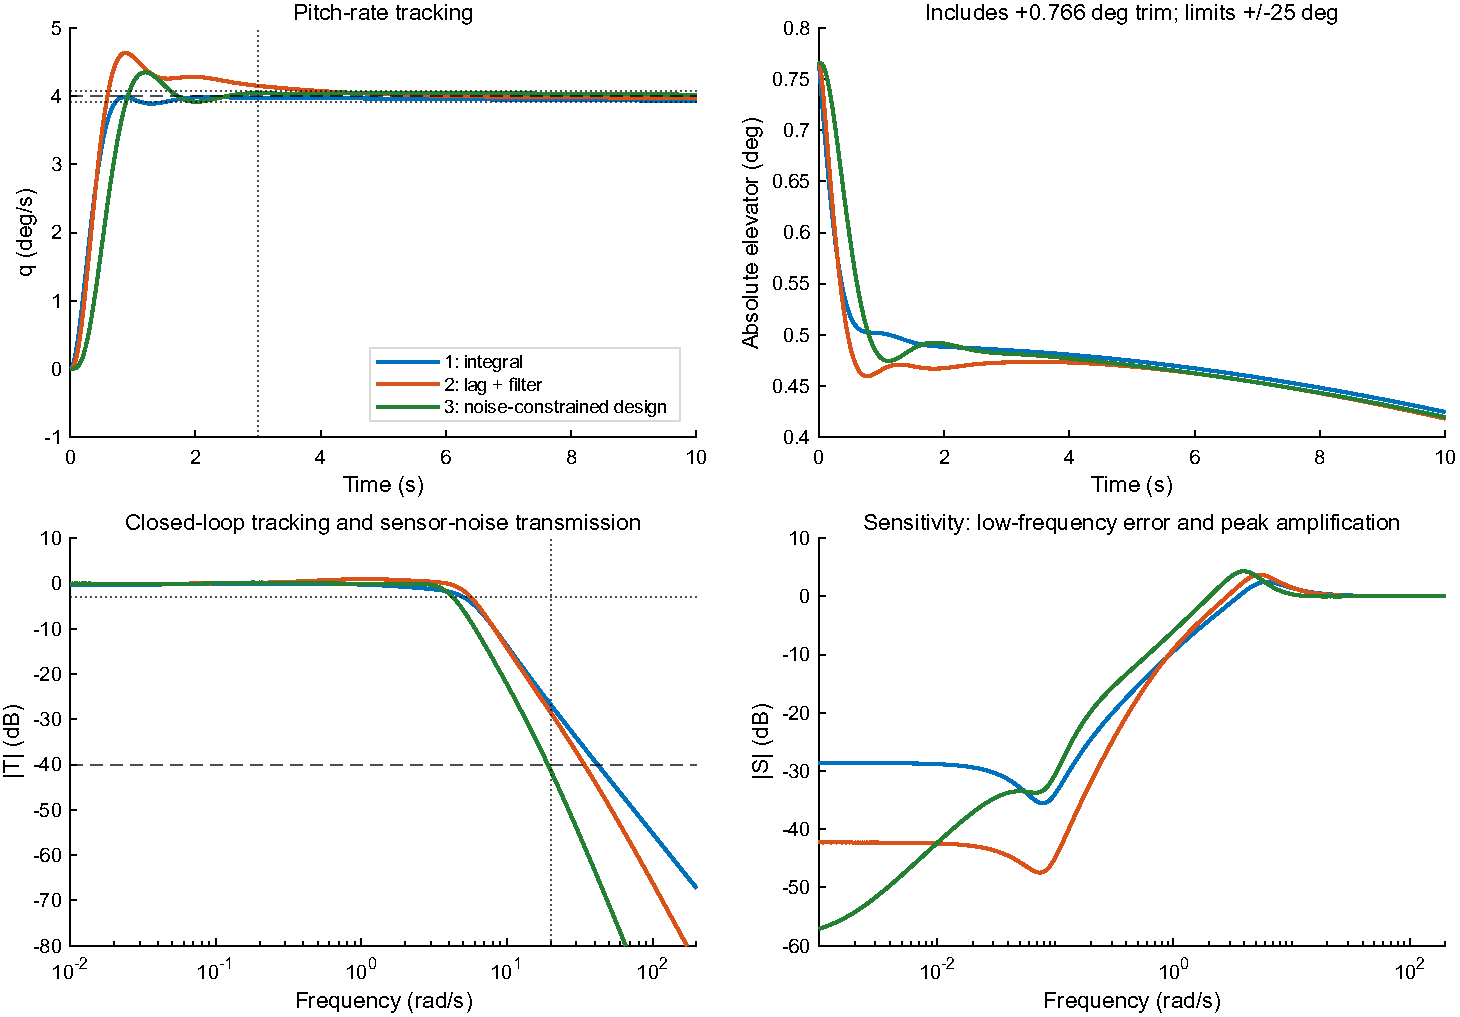
\includegraphics[width=1.0\linewidth]{comparison.pdf}\caption{Tracking, absolute elevator, complementary sensitivity and sensitivity.}\end{figure}


\clearpage\section{Engineering Validation}
\subsection{Airspeed}
The nonlinear model was retrimmed at 180 and 210 knots by solving for level-flight angle of attack, throttle and elevator at 300 ft. Central-difference Jacobians were recomputed with the controller fixed. Throttle remains within $[0,1]$ and trim residuals are below $10^{-6}$.
\begin{table}[H]\centering\small\caption{Fixed controller at separately verified trim points.}
\begin{tabular}{lrrrrr}\toprule
Speed (kt) & Throttle & SSE (\%) & OS (\%) & $t_s$ (s) & $\omega_{BW}$\\\midrule
180 & 0.570 & 0.172 & 7.051 & 1.703 & 3.824\\
200 & 0.770 & 0.116 & 8.897 & 1.607 & 4.237\\
210 & 0.887 & 0.097 & 9.823 & 1.999 & 4.435\\
\bottomrule\end{tabular}\end{table}

All three sampled points meet the main time-domain and noise targets.

\subsection{Actuator and Delay}
Servo and sensor dynamics are unspecified. Separate actuator sensitivity tests assume $A_e(s)=1/(1+\tau s)$:
\begin{table}[H]\centering\small\caption{Assumed first-order actuator dynamics.}
\begin{tabular}{lrrrr}\toprule
$\tau$ (s) & SSE (\%) & OS (\%) & $t_s$ (s) & PM (deg)\\\midrule
0.000 & 0.116 & 8.897 & 1.607 & 60.301\\
0.025 & 0.116 & 12.377 & 2.275 & 57.460\\
0.050 & 0.116 & 15.878 & 2.451 & 54.738\\
0.100 & 0.116 & 22.314 & 3.757 & 49.748\\
\bottomrule\end{tabular}\end{table}

The 50 ms case passes the main step targets. The 100 ms case is stable but exceeds the settling and overshoot limits. Airspeed and actuator cases were tested separately.

Pure delay reduces phase margin by $\omega_{gc}\tau_d$ radians. Nominal delay margin is 0.522 s; 10--40 ms cases are in \file{delay.csv}. Position limiting and conditional integration are implemented [4]. The test manoeuvres remain below the position and assumed 60 deg/s rate limits, so saturation recovery remains untested [5].

\subsection{Uncertainty and Digital Implementation}
Pitch stiffness $A_{32}$, damping $A_{33}$ and elevator effectiveness are varied independently by $\pm20\%$. All 27 minimal q channels remain stable; 21 meet all time-domain targets and 18 meet the noise criterion. Overshoot spans 1.49--33.37\%, settling 1.07--3.28 s, and phase margin 39.00--73.41 deg.

At 100 Hz, a ZOH plant and Tustin controller give tracking bandwidth 4.258 rad/s and maximum dynamic pole magnitude 0.999423949. The unreduced discrete system retains a neutral pole at $z=1$. Hardware latency, quantisation, jitter and anti-alias filtering remain implementation inputs.
\begin{figure}[H]\centering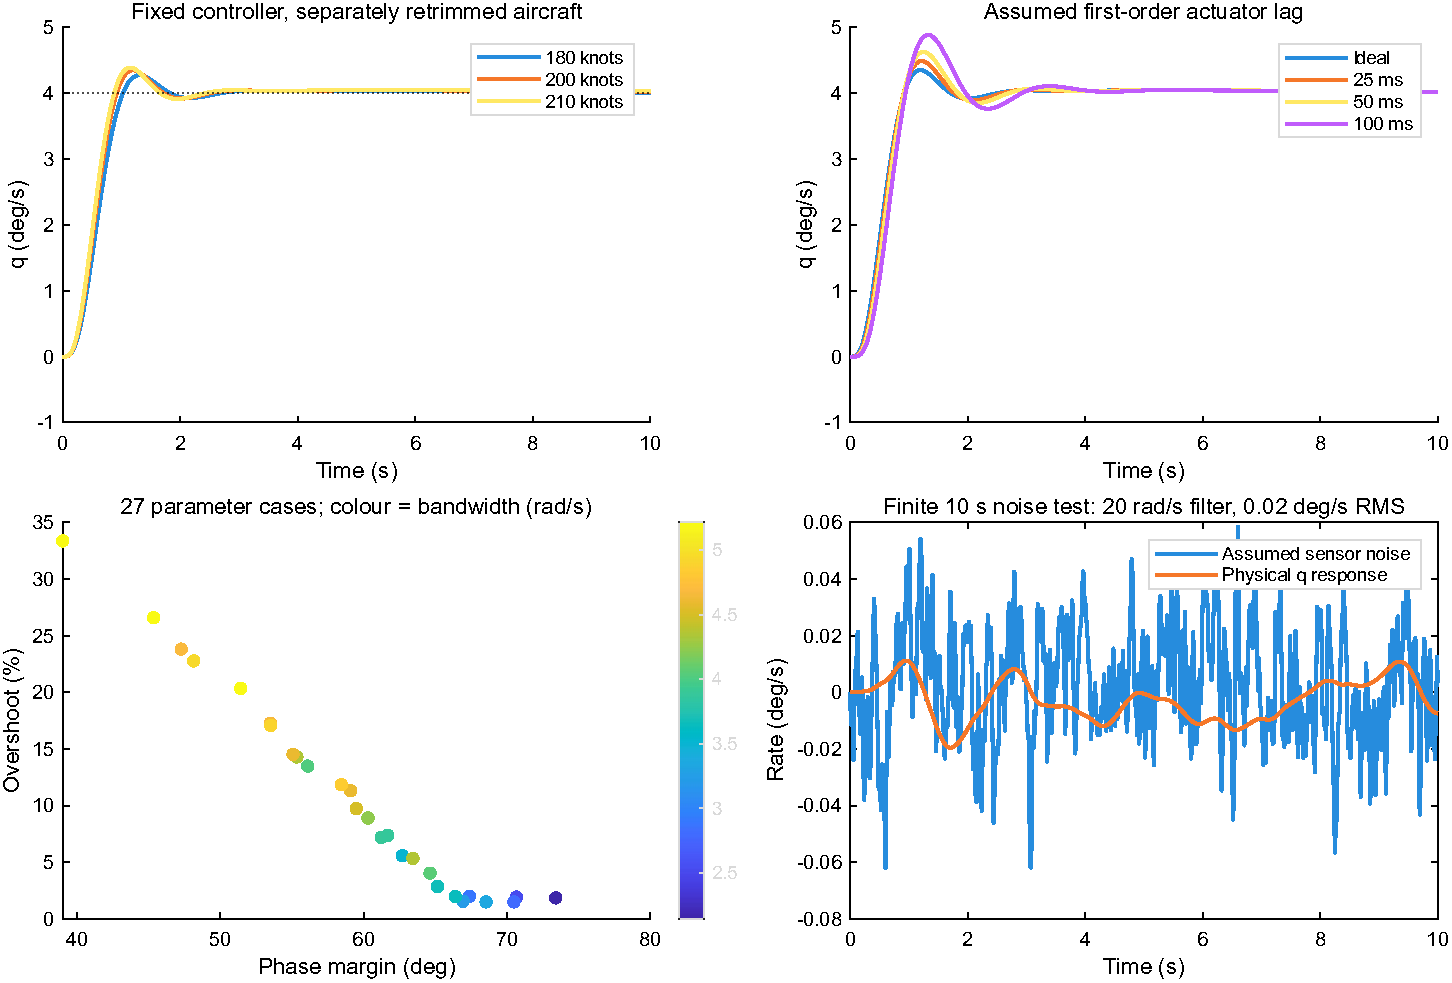
\includegraphics[width=1.0\linewidth]{robustness.pdf}\caption{Separate speed, actuator, parameter and finite-noise checks.}\end{figure}


\clearpage\section{Nonlinear Response and Internal Dynamics}
The unreduced aircraft/controller system has one zero eigenvalue; all remaining eigenvalues have negative real parts. Because $\dot\theta=q$, sustained nonzero q produces a pitch-angle ramp. The origin pole in $U=K_qS$ also permits control drift under persistent commands or sensor bias. Stable q tracking therefore requires attitude and command management in the outer loop.

The supplied 12-state nonlinear model uses converged implicit aerodynamic rates. A 5 s ideal-actuator step differs from the linear q response by at most 0.0403 deg/s. For a 2 s rate pulse:
\begin{itemize}
\item Peak q: 4.3476 deg/s; peak absolute elevator: 0.7732 deg; peak rate: 0.478 deg/s.
\item Maximum pitch angle: 8.408 deg; minimum speed: 93.874 m/s with fixed throttle.
\item Peak body-normal load: 1.759 g; maximum linear/nonlinear q difference: 0.0314 deg/s.
\end{itemize}
At 200 knots and 4 deg/s, $Vq/g\approx0.73$, explaining the significant normal-load increment despite small elevator motion. Stall and structural margins require $C_{L\max}$ and load-limit data. Speed loss motivates auto-throttle integration.
\begin{figure}[H]\centering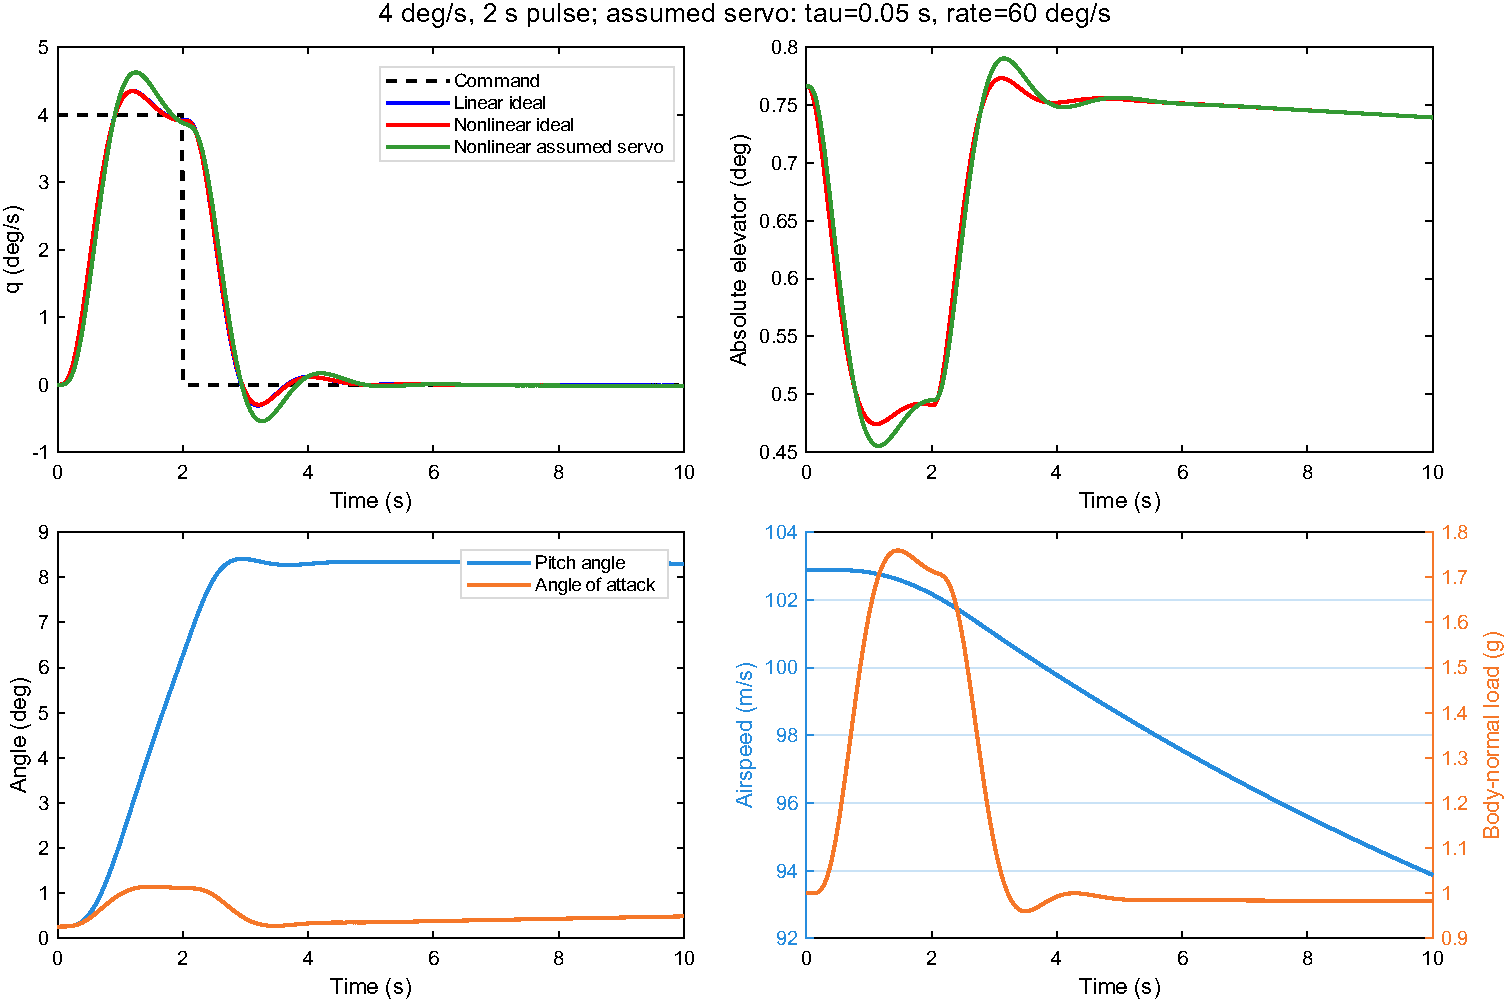
\includegraphics[width=1.0\linewidth]{nonlinear.pdf}\caption{Finite pitch-rate pulse; assumed actuator is 50 ms and 60 deg/s.}\end{figure}


\subsection{Measurement Noise}
A 10 s sensor-noise test assumes 0.02 deg/s RMS and a 20 rad/s low-pass filter. Physical q RMS is 0.00804 deg/s and elevator-increment RMS is 0.000547 deg. Nominal $|T(j20)|=-41.41$ dB. The one-sided equivalent area $\int_0^\infty|T(j\omega)/T(0)|^2d\omega$ is 4.477 rad/s. Elevator RMS is specific to this finite record because its path retains an integrator.

\section{Reproduction and Next Steps}
From the assignment root:
\begin{verbatim}
run('inner_loop/run_inner.m')
open_sisotool(3)
\end{verbatim}
The first command rebuilds controllers, validation, ZPK exports and plots; the second opens the selected SISOtool model. Keep the adjacent \file{Gqde}, \file{A_B_Matrix} and \file{trim} folders. GUI steps are normalised; numerical tests use the physical 4 deg/s input in radians.

The design uses Lectures 4--5 (frequency response and modal scales), 8 (root locus, margins and compensation), 9 (aircraft control structure and digital implementation), and 10 (integrator placement, sign and SCK form). Lectures 6--7 and 11 support the later stochastic gust analysis.

Next derive $q_c\rightarrow V_s$ and design the vertical-speed loop, followed by auto-throttle, Dryden gust analysis and full integration.

\section*{References}
\addcontentsline{toc}{section}{References}
\begin{enumerate}
\item MathWorks, \href{https://www.mathworks.com/help/control/ref/dynamicsystem.bandwidth.html}{bandwidth: frequency response bandwidth}.
\item MathWorks, \href{https://www.mathworks.com/help/control/ref/dynamicsystem.margin.html}{margin: gain/phase margins and crossover frequencies}.
\item MathWorks, \href{https://www.mathworks.com/help/control/ug/bode-diagram-design.html}{Bode diagram design}, and \href{https://www.mathworks.com/help/control/ref/controlsystemdesigner-app.html}{Control System Designer}.
\item MathWorks, \href{https://www.mathworks.com/help/simulink/slref/anti-windup-control-using-a-pid-controller.html}{Anti-windup control using PID Controller block}.
\item R. A. Hess and S. A. Snell, \href{https://ntrs.nasa.gov/citations/19980017538}{Flight Control System Design with Rate Saturating Actuators}, NASA/CR-97-207117, 1997.
\item AERO5560 Group Project, Longitudinal Task 1, pp. 2--3; Lectures 4, 5, 8, 9, 10 and 11, supplied course material. Aircraft data: Group 8 Canvas package.
\end{enumerate}
\end{document}
